\section{Discussion}
\label{sec:discussion}

\subsection{What is different about a millimetre technosignature search}
\label{sec:mmdifferent}

The most transferable result of this experiment is not the non-detection. It
is a measurement of what actually limits a carrier search at millimetre and
submillimetre wavelengths. The binding constraints are molecular-line
confusion, a channelisation chosen by other observers for other purposes, and
when the archive happened to look. Thermal sensitivity, which is what usually
limits a centimetre-wave search, is not among them: ALMA supplies more of it
than this experiment can use.

\emph{Confusion, and not interference, sets the false-positive rate.}
Catalogued molecular transitions, almost all of them carbon monoxide, account
for \NAttributed{} of the \NCross{} threshold crossings, and no crossing in
this survey is attributed to interference (Appendix~\ref{app:rfi}).
\DiscFpWin{} of the \DiscFpOfFlags{} windows that reached the spatial stage
are disc or foreground carbon monoxide, arising in \DiscFpSys{} of the
\NDebrisKwSys{} debris-disc systems searched. The remedy that works is a
velocity-space mask evaluated in the stellar frame, and it is not free: it
removes \MaskLostPct{} per cent of otherwise usable coverage.

\emph{Spatially extended emission is the second discriminant, and it has no
real analogue at centimetre wavelengths.} A line that fills the primary beam
raises the star and the control annulus together instead of cancelling, so
the spatial screen loses power exactly where circumstellar gas is brightest.
Two targets show both faces of this. $\beta$~Pictoris is the benign one: the
frozen pipeline recovers its circumstellar carbon monoxide blind, in two
transitions, which is the positive control the experiment needed. HD~48370 is
the awkward one. Its resolved disc emission lies close to a band edge, and
that single window contributes \VnEdgeDomPct{} per cent of all the near-edge
threshold exceedances in the survey. Pooled over the searched windows the
near-edge exceedance rate is $\times\VnEdgeRatio$ the interior rate; drop that
one window and it is $\times\VnEdgeNoDomRatio$, and on the half of the windows
held out from its own stratum it is $\times\VnEdgeHalfCleanRatio$
($\pv{\VnEdgeHalfCleanP}$). What looked like a property of the band edges is
one resolved disc, so no edge correction is applied to any limit.

\emph{The channelisation is inherited, and it decides what kind of search is
possible at all.} \NCoarse{} of the \NWindows{} windows searched have channels
so coarse that every drift in the grid stays within one channel over a whole
track; they measure an amplitude but cannot tell a drifting carrier from a
stationary one, which is why the carrier search rests on \NWinA{} of them.
Across the archive the native channel widths span about seven orders of
magnitude (Fig.~\ref{fig:context}(b)), and nothing in the search could choose
them.

\emph{Repeat epochs are what turn a crossing into a candidate, and an archive
supplies them only incidentally.} Temporal sampling is the weakest axis of
this experiment, and for close to half the sample it constrains an
intermittent emitter hardly at all, whatever its power. Coverage is also
incomplete at the level of whole observations: \FateDone{} of the
\FateScope{} execution blocks in scope were searched, \FateNoCal{} carry no
observatory calibration at all, \FateCalFail{} failed calibration,
\FateInfeas{} is infeasible at this data volume and \FateUnattempted{} were
not attempted. For one of them the observatory delivered raw data it had
never calibrated, so part of that gap lies in the delivery rather than in the
processing.

\emph{Finally, a threshold is not a sensitivity, and here the difference is
large.} A nominal trigger level is a property of the noise, not a statement
about what a transmitter of a given power does to a pipeline. Measured by
injection and recovery through the complete automated selection, the power
needed for 90 per cent recovery is $\StrMultNoise$ times the trigger power in
the Class~A windows whose control ring is noise, more than $\StrPosCtrl$
times it in the \StrNDiscWin{} whose ring carries resolved emission, and
$\EirpNinetyMultB$ times it in Class~B. One limitation should be read
with every number here: every check reported in this paper tests this
pipeline against itself, and because the only other archival search at these
frequencies targets a disjoint sample, there is no external pipeline to
compare against.

\subsection{The search space this archive opens}
\label{sec:newspace}

The carrier search is \NWinA{} fine-channel windows toward \NSysClassA{}
stellar systems, covering \DnuA\,GHz of unique sky frequency; the \NWinB{}
coarse-channel windows are a supplementary spectral-excess experiment that
cannot search for drift at all. Three statements about novelty are worth
keeping apart, because they are easily run together. No previous search has
looked for technosignatures toward stars within 40\,pc at any frequency above
about 30\,GHz. One previous search has worked in ALMA Band~3, but toward
stars at \MasonNearKpc\,kpc and beyond \citep{Mason2025}, so Band~3 is not
searched toward nearby stars either. And \UnionBandThree\,GHz of the frequency
covered here lies inside the 10\,MHz--115\,GHz interval that
\citet{Wright2018} adopt as the frequency axis of the search haystack, which
is a definition of parameter space rather than coverage by any telescope.

Bandwidth alone overstates what that buys, because different frequencies were
searched toward different numbers of stars and to very different limits.
Figure~\ref{fig:covmap} therefore replaces \DnuA\,GHz as the
description of coverage with the quantity a reader needs: how many
independent systems would have yielded a recovery at 90 per cent
completeness, as a function of sky frequency and transmitter power. At an
EIRP of $\CovEirpRefTex$\,W the covered frequency falls to
\CovUnionAtRef\,GHz, \CovFracAtRef{} per cent of the union, reaching
\CovNSysAtRef{} systems in all and \CovNMaxAtRef{} at the best-covered
frequency near \CovNuMaxAtRef\,GHz. With no limit on power that same
frequency reaches \CovNMaxFull{} of the \NSysClassA{} systems, and half the
sample is reached only above $\CovEirpHalf$\,W.

\begin{figure}
\centering
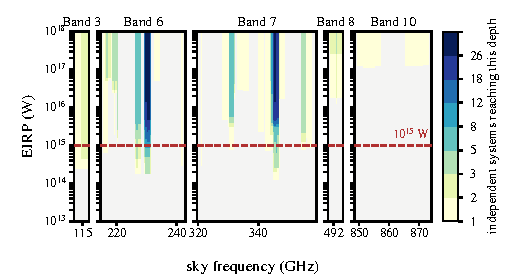
\includegraphics[width=\columnwidth]{figures/completeness_map.pdf}
\caption{Where the experiment could have found something. Shading gives the
number of independent systems that would have yielded a recovery at 90 per
cent completeness for an unresolved carrier of the plotted EIRP at the
plotted sky frequency; unshaded means none. One panel per populated ALMA
band, with panel widths in proportion to the frequency each contributes: the
\DnuA\,GHz of Class~A coverage is \CovNIslands{} disjoint islands spread
across \DomAFreqLo--\DomAFreqHi\,GHz, so a single continuous abscissa would
draw every island as a hairline. The dashed line is $\CovEirpRefTex$\,W, at
which \CovUnionAtRef\,GHz of the union survives.
Figure~\ref{fig:waterfall} shows where ALMA looked; this shows where the
experiment was sensitive.}
\label{fig:covmap}
\end{figure}

\emph{Archival SETI buys sky and frequency cheaply and buys confirmation not
at all.} Across both classes this experiment reached \NSystems{} systems and
\UnionGHz\,GHz without an allocation, at a sensitivity no targeted programme
at these frequencies has matched, on data selected by others.
\PctDiscProposal{} per cent of the searched stars were observed for disc or
planet-formation science, which puts circumstellar carbon monoxide in a large
fraction of the fields, and \SfMSearched{} of the \SfMCensus{} catalogued
M~dwarfs within 40\,pc have any coverage at all
(\S\ref{sec:bias}). The quantities here describe
\emph{these} stars, frequencies and epochs and nothing wider.

For comparison with other programmes the conventional measure is the
continuous-waveform transmitter figure of merit of \citet{Enriquez2017},
$\mathrm{CWTFM}=\zeta_{\rm AO}\,\mathrm{EIRP}_{\rm min}/
(N_{\star}\nu_{\rm rel})$, in which $\nu_{\rm rel}=\Delta\nu/\nu_{\rm mid}$ is
the fractional bandwidth and $\zeta_{\rm AO}$ is fixed so that the merit is
unity for \FomNormN{} stars at $\nu_{\rm rel}=\FomNormNuRel$ and an EIRP of
$\FomAreciboEirp$\,W; smaller is better. For the Class~A experiment
$N_{\star}=\NSysClassA$ and $\nu_{\rm rel}=\FomNuRel$, and taking
$\mathrm{EIRP}_{\rm min}$ as the largest in the sample, which is the
convention, the value is $\FomCwtfmWorst$ --- on the median rather than the
worst system, $\FomCwtfmMed$. \citet{Enriquez2017} report \FomLitEnriquez,
and \citet{Margot2023} correspond to \FomLitMargot, evaluated here from their
published sample size, band and power limit because that paper reports a
modified Drake figure of merit instead. Nearly all of the difference is the
product $N_{\star}\nu_{\rm rel}$: \NSysClassA{} systems across a fractional
bandwidth of \FomNuRel{} is a far smaller haystack than a wideband centimetre
survey of thousands of stars, and the Drake figure of merit is dominated by
instantaneous bandwidth in the same way. Both compare surveys; neither is an
occurrence rate, and the non-detection here cannot be converted into one
because an archive-selected sample does not supply the denominator.

\subsection{What this experiment excludes, and what it does not}
\label{sec:excludes}

\noindent\emph{Excluded.} Consider a continuously transmitting, unresolved
carrier that lies outside the molecular-line mask, inside the searched
frequency range and inside the linear-drift grid, and that is present during
one of the archival epochs. Such a carrier would have been found nine times
in ten above the $\mathrm{EIRP}_{90}$ of \S\ref{sec:pninetysel}, a median of
$\EirpNinetySysMedA$\,W per system on its best window. None is present toward
any of the \NSysClassA{} systems the carrier search covers.

Four further axes bound the excluded population as sharply as power does.
\emph{Frequency:} the coverage is sparse and inherited, and
Fig.~\ref{fig:covmap} is the statement of it; the median system is covered
over only \SysUnionAMed\,GHz. \emph{Drift and acceleration:} the searched grid
reaches a line-of-sight acceleration of
\AccelCeilMed--\AccelCeilMax\,m\,s$^{-2}$, which contains every known planet
of the sample but one (Fig.~\ref{fig:accel}). A transmitter whose own
oscillator drifts faster than that kinematic budget lies outside the grid.
\emph{Persistence:} the carrier must be radiating during one of the
archival observations, so these are limits on persistent emission.
\emph{Spectral width:} the statistic is built for emission confined to one
\ChanLoA--\ChanHiA\,kHz channel. A carrier broadened beyond a channel loses
signal to its own width, and a signal broad enough to resemble continuum is
removed with the spectral baseline.

\noindent\emph{Not excluded.} A transmitter absent during the archival
observation, or on for less than about a tenth of the time. At a duty cycle
of one tenth, recovery falls
to \DwellFineT{} per cent for the fine class and \DwellCoarseT{} for the
coarse; those trials are undrifted, so the joint drifting-and-intermittent
case is not measured at all. Emission inside the
$\pm\MaskHalfKms$\,km\,s$^{-1}$ molecular-line mask, at any strength, which
costs \MaskLostGHz\,GHz of coverage. Drift outside the searched grid, or
drift curved enough to leave a channel within the track. Signals broad enough
to be removed with the continuum baseline. Anything below a window's own
completeness. And any emission from the \NGaiaCensus{} stars within 40\,pc
that ALMA has not observed, which is almost all of them.

\noindent\emph{An illustrative engineering benchmark.} A limit of
$10^{15}$\,W is hard to picture, so it is worth naming one transmitter that
would produce it, provided the example is not mistaken for a privileged
scale. A \BenchDiam\,m dish radiating \BenchPowerMW\,MW at \BenchFreqGHz\,GHz
at an aperture efficiency of \BenchEta{} has a directive gain
$G=\eta(\pi D\nu/c)^{2}=\BenchGain$ and so an EIRP of $\BenchEirp$\,W, a
depth this survey reaches for \BenchNSysA{} of the \NSysClassA{} Class~A
systems. Nothing but convenience selects those numbers --- aperture,
efficiency, pointing, duty cycle and the chance that the beam contains the
Solar System all enter, and none is constrained here --- so the results of
this paper remain the model-independent $\mathrm{EIRP}_{90}$ limits. What the
example does make plain is that EIRP is not transmitter power: the same
megawatt radiated isotropically would be $10^{6}$\,W of EIRP, and it is the
directivity that lifts a modest transmitter into the range this survey
probes. These limits therefore apply to beamed transmitters whose beam
contains the Solar System, and say almost nothing about omnidirectional
beacons.

\noindent\emph{Two blind spots.} The search is Stokes~$I$ only, so the
discrimination that polarisation would offer against unpolarised
astrophysical emission is unavailable; ALMA's feeds are linear, and the
circularity of a circularly polarised carrier lies in the cross-hands, which
this analysis does not extract. And the frequency coverage is the archive's
and not a choice: none of the ``magic frequency'' arguments that have guided
centimetre-band searches falls in an ALMA band, so a transmitter deliberately
placed on one lies outside this experiment by construction.

\subsection{What a dedicated ALMA technosignature experiment should do
differently}
\label{sec:future}

A purpose-built experiment on the same telescope would be far stronger, and
the changes it needs follow from the limitations above. \emph{Channelise
finely everywhere:} the \NCoarse{} coarse-channel windows measure an amplitude
but cannot distinguish a drifting carrier from a stationary one.
\emph{Choose the targets and the frequencies:} an archive weighted toward
dusty discs is the worst case for molecular-line confusion, the M~dwarfs that
dominate the nearby habitable-zone planet census are the least covered, and
windows placed deliberately away from the bright transitions would recover
most of the \MaskLostGHz\,GHz the mask costs --- all three are decisions a
proposal can simply reverse. \emph{Repeat the epochs on purpose:} two or
three visits separated by days and by years turn a crossing into a testable
claim, and the separation is a scheduling constraint rather than extra
sensitivity. \emph{Keep the controls and the polarisation:} full dynamic
spectra survive for only \LNNRetained{} of the \NCtrl{} control positions
here, which is what limits the second-stage null in a structured field, and
only a cross-hand extraction can see a circularly polarised carrier; both cost
storage and nothing else. \emph{Retain the visibilities:} rotating the phase
centre to the star leaves a genuine point source entirely in the real part of
the visibility, with an imaginary part consistent with zero on every
baseline. That asks whether the data contain a source \emph{where the star
is} --- a physically specific question, and a stronger one than any rank
against neighbouring positions in an image.

%% ---------------------------------------------------------------------
%% REQUEST (06_discussion owner -> integrator). Consequences of this pass.
%% None of them is in a file I own; each is also written up as a numbered
%% entry in referee_r10/INTEGRATION_QUEUE.md.
%%
%% Q1. LABELS. sec:newspace, sec:excludes and sec:discussion are unchanged.
%%     sec:exposure and sec:parallax are GONE (see Q2, Q3); no file refers
%%     to either. sec:lessons is renamed sec:mmdifferent; the benchmark is
%%     a labelled paragraph inside sec:excludes, which is where \S2 now points.
%% Q2. THE OMITTED ANNUAL PARALLAX subsection is deleted from the Discussion
%%     under the ruling that the correction is applied rather than stated.
%%     The statement must now be made exactly once, where it is applied, in
%%     Section 5.1 / Appendix A. Macros \PxNWin, \PxLossMedPct,
%%     \PxLossMaxPct, \PxNGtTen and \PxNSysCorr are no longer referenced by
%%     any file I own and retire_macros.py will drop them unless that
%%     statement cites them.
%% Q3. THE ON-SOURCE TIME subsection (two offsetting bookkeeping biases) is
%%     deleted here as reproducibility detail. It belongs in Appendix A.
%%     Macros \TruncNBlocks, \ExpNBlocks, \TruncNWin, \TruncNStars,
%%     \TruncHoursLost, \TruncPctSurvey, \TruncGainMed, \OcOldMax,
%%     \OcNewMax, \ExpNetLo, \ExpNetHi are orphaned by that deletion.
%% Q4. THE MASON MATCHED-RECEIVED-FLUX COMPARISON is now made once, in
%%     Section 2, as that section's own request asked. \FluxSelMatchMed and
%%     \FluxSelMedRatio are unused.
%% Q5. THE BENCHMARK must stop being quoted as a headline result elsewhere:
%%     it is now an explicitly illustrative example in Section 6.3.
%%     Remove it from the abstract, from Section 5 and from conclusion 3,
%%     each of which should quote the EIRP_90 limit alone.
%% Q6. CONCLUSION 1 states that \UnionBandThree GHz of the searched range
%%     lies inside the interval covered by centimetre-wave programmes. It
%%     does not; that is the Band 3 union inside the Wright et al. haystack
%%     AXIS. Replacement text is in the integration queue.
%% Q7. Figure fig:covmap is new and is paid for: the millimetre-motivation
%%     paragraph (duplicated from Section 1), the Mason flux comparison, the
%%     parallax subsection and the exposure subsection are all deleted here.
%% ---------------------------------------------------------------------
